The muon control region ($\crwmn$) is used to estimate the $\wmunuplusjets$ and
the $\znunuplusjets$ background contribution in the SR\@. The $\wmunuplusjets$
events can enter the SR if the muon is outside the detector acceptance or it
fails quality criteria. $\wmunuplusjets$ events are selected and used in order
to estimate the $\znunuplusjets$ contribution in the signal region. The muon is
treated like a neutrino in the $\met$ calculation, in this way the $\met$ is a
measurement of the $W$ momentum which is later translated in the $Z$ boson
momentum to estimate the $\znunuplusjets$ background. The CR$_{\mathrm{\, wmn}}$
region selects events with:
\begin{itemize}
\item Exactly one good muon.
\item The transverse mass, defined as:
  \begin{equation}
    \label{eq:82}
    m_\mathrm{\, T} = \sqrt{2 p_\mathrm{\, T}^{\, \mu} p_\mathrm{\, T}^{\, \nu}
      (1 - \cos(\phi_\mu - \phi_\nu))}
  \end{equation}
  and determined by the muon $\pt$ ($\pt^{\, \mu}$) and neutrino $\pt$
  ($\pt^{\, \nu}$), is required to be $30~<~m_\mathrm{\, T}~<~100$~GeV,
  consistent with $W$ boson production. The neutrino $\pt$ is calculated
  assuming that $\pt^{\, \nu} = \met$.
\end{itemize}
The transverse mass cut suppress the $\wtaunuplusjets$ processes in this
region. The measured $\met$ and leading jet $\pt$ distributions after the
fitting the background normalizations to the control regions (see
\cref{sec:glob-simult-likel}) are shown in Figure~\ref{fig:muon_cr_plots}. The
agreement between data and MC is good.
\begin{figure}[!h]
  \centering
  \begin{subfigure}[t]{.48\linewidth}
    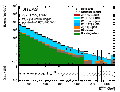
\includegraphics[width=\linewidth]{muon_cr_et_miss_post_fit}
    \caption{$\met$ distribution.}
    \label{fig:muon_cr_et_miss_pre_fit}
  \end{subfigure}
  \begin{subfigure}[t]{.48\linewidth}
    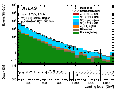
\includegraphics[width=\linewidth]{muon_cr_jet1_pt_post_fit}
    \caption{Leading jet $\pt$ distribution.}
    \label{fig:muon_cr_jet1_pt_pre_fit}
  \end{subfigure}
  \caption{Observed and predicted $\met$ and leading jet $\pt$ distributions
    after the background only fit in the single muon $\crwmn$ for the
    $\met > 250~$GeV selection. The error bands include the statistical and
    systematic error.}
  \label{fig:muon_cr_plots}
\end{figure}
%%% Local Variables:
%%% mode: latex
%%% TeX-master: "../search_for_DM_LED_with_ATLAS"
%%% End:
